%%
%% This is the converted project report in the acmart sigconf format.
%%
\documentclass[sigconf, screen]{acmart}

%%
%% Custom packages from the original report that are still needed.
%% acmart already loads graphicx, booktabs, hyperref, amsmath, xcolor.
\usepackage{float}       % For the [H] option on floats
\usepackage{fancyvrb}    % For the Verbatim environment in the appendix
\usepackage{fvextra}   
\usepackage{subcaption}  % For subfigures if needed, although not used in the final example
\usepackage{fancyhdr}
\usepackage{algorithm} 
\usepackage{algpseudocode}

\fancypagestyle{ack_footer}{
    \fancyhf{}
    \renewcommand{\headrulewidth}{0pt}
    \renewcommand{\footrulewidth}{0pt}
    \cfoot{
      \scriptsize
      \begin{minipage}[t]{0.95\textwidth}
      \textbf{AI Acknowledgments:} OpenAI's ChatGPT (model gpt-4o) was utilized to generate code from formulas and algorithms, assist in generating the visualization script to create plots from results, adding comments where needed, to help debug code and set up errors, and assist in \LaTeX formatting. The outputs from this AI model were modified with \textbf{major changes} to align with assignment requirements and ensure correctness. I actively reviewed, tested, and adjusted the generated code and explanations to reflect my own understanding.
      \end{minipage}
    }
}

%%
%% \BibTeX command to typeset BibTeX logo in the docs
\AtBeginDocument{%
  \providecommand\BibTeX{{%
    Bib\TeX}}}

%% Rights management information.
\setcopyright{none}
\copyrightyear{2025}
\acmYear{2025}
\acmDOI{XXXXXXX.XXXXXXX}

%% Conference information
\acmConference[CSE 240A Project]{CSE 240A Branch Predictor Project Report}{Spring 2025}{UC San Diego}
\acmBooktitle{CSE 240A Branch Predictor Project Report, Spring 2025, UC San Diego}
\acmISBN{}

%%
%% These commands remove the ACM reference format and permissions block,
%% and add page numbers, which is more suitable for a project report.
\settopmatter{printacmref=false}
\settopmatter{printfolios=true}
\renewcommand\footnotetextcopyrightpermission[1]{}
\pagestyle{plain}


%%
%% end of the preamble, start of the body of the document source.
\begin{document}

%%
%% The "title" command
\title{CSE 240A Branch Predictor Project: G-Share, Tournament, and a Custom TAGE Implementation}

%%
%% The "author" command
\author{Param Somane}
\authornote{Project code repository: \href{https://github.com/ChestnutKurisu/CSE240A_Branch_Predictor_SP25/}{github.com/ChestnutKurisu/CSE240A\_Branch\_Predictor\_SP25}}
\affiliation{%
  \institution{Department of Computer Science and Engineering}
  \institution{University of California, San Diego}
  \city{La Jolla}
  \state{CA}
  \country{USA}
}
\email{psomane@ucsd.edu}


%%
%% The abstract is a short summary of the work to be presented in the
%% article.
\begin{abstract}
Branch prediction is a critical optimization in modern CPU microarchitecture, allowing processors to speculatively execute instructions beyond unresolved conditional branches, thereby hiding pipeline latency and improving instruction throughput. This project implements and evaluates three distinct branch predictors: G-Share, Tournament, and a custom TAGE-based predictor, all integrated within a common simulation framework. We present a detailed analysis of their design, implementation trade-offs, experimental observations on six benchmark traces, and final performance results. The custom TAGE predictor, leveraging multiple tagged tables with varying history lengths, achieves the highest accuracy, significantly outperforming the simpler G-Share and Tournament schemes. We also analyze the memory footprint of each predictor to ensure compliance with the project's 64K+256-bit constraint, demonstrating a practical approach to designing hardware-conscious predictors.
\end{abstract}


%%
%% This command processes the author and affiliation and title
%% information and builds the first part of the formatted document.
\maketitle

\section{Introduction}
Modern processors rely on deep instruction pipelines to achieve high clock frequencies and performance. However, the effectiveness of these pipelines is severely hampered by control hazards, which arise from conditional branch instructions. When a branch is encountered, the processor must determine its outcome (taken or not-taken) and target address before it can fetch the next correct instruction. A wrong fetch stalls the pipeline, requiring a flush of all speculatively fetched instructions, which can waste dozens of cycles and significantly degrade performance.

\emph{Branch prediction} is a microarchitectural technique designed to mitigate this penalty. By predicting the outcome of a branch before it is executed, the processor can speculatively fetch and execute instructions along the predicted path. An accurate prediction avoids pipeline stalls, while a misprediction still incurs the cost of a pipeline flush. The goal of a branch predictor is thus to maximize the prediction accuracy, a challenge explored in early seminal works like that of Smith \cite{yhsmith1981}, while adhering to strict hardware budget constraints (in terms of area and power).

In this project, we explore the design and performance of three progressively sophisticated branch predictors:
\begin{itemize}
    \item \textbf{G-Share:} A classic predictor that correlates global branch history with the branch address.
    \item \textbf{Tournament:} A hybrid predictor that dynamically selects between a local and a global predictor, adapting to the dominant correlation patterns in the workload.
    \item \textbf{Custom (TAGE-like):} An advanced, state-of-the-art predictor that uses multiple tagged tables with geometrically increasing history lengths to capture both short- and long-term correlations.
\end{itemize}

This report details the implementation of each predictor, followed by a thorough experimental evaluation using six benchmark traces representing diverse workloads (integer, floating-point, and memory-intensive). We analyze misprediction rates and memory usage, culminating in a comparative study that highlights the strengths and weaknesses of each approach. The findings confirm that the increased complexity of the TAGE predictor yields substantial improvements in accuracy, justifying its adoption in high-performance processors.

\section{Implementation}

This section details the working principles, data structures, and algorithmic logic for each of the three implemented predictors. All predictors were constrained to a total memory budget of 64KB + 256 bits. We also briefly discuss the historical evolution of each technique.

\subsection{G-Share Predictor}

\subsubsection{High-Level Concept}
The G-Share predictor \cite{mcfarling1993combining} evolved from earlier two-level global predictors to solve the problem of destructive aliasing. Simple global predictors used a Global History Register (GHR) to index a table of counters, but unrelated branches could map to the same entry and interfere. G-Share mitigates this by creating an index through a simple hash: it XORs the lower bits of the Program Counter (PC) with the GHR. This mixing of PC and history helps to differentiate branch patterns that would otherwise collide, leading to higher accuracy.

\subsubsection{Algorithm and Data Structures}
The core data structures are a GHR and a Branch History Table (BHT).
\begin{itemize}
    \item \textbf{Global History Register (GHR):} An $N$-bit shift register that stores the outcomes of the last $N$ branches.
    \item \textbf{Branch History Table (BHT):} An array of $2^N$ 2-bit saturating counters. Each counter can be in one of four states: Strongly Not-Taken (SN), Weakly Not-Taken (WN), Weakly Taken (WT), or Strongly Taken (ST).
\end{itemize}
The prediction and training logic is outlined in Algorithm \ref{alg:gshare}. The key operation is the index calculation, which is a bitwise XOR.

\begin{algorithm}[H]
\caption{G-Share Prediction and Training}
\label{alg:gshare}
\begin{algorithmic}[1]
\Statex \textbf{Data Structures:}
\State $GHR$: Global History Register of length $N$
\State $BHT$: Table of $2^N$ 2-bit saturating counters, initialized to WN
\Statex
\Procedure{Predict}{$PC$}
    \State $mask \gets (1 \ll N) - 1$
    \State $index \gets (PC \land mask) \oplus (GHR \land mask)$
    \State $counter \gets BHT[index]$
    \If{$counter \ge WT$}
        \State \textbf{return} TAKEN
    \Else
        \State \textbf{return} NOTTAKEN
    \EndIf
\EndProcedure
\Statex
\Procedure{Train}{$PC, outcome$}
    \State $mask \gets (1 \ll N) - 1$
    \State $index \gets (PC \land mask) \oplus (GHR \land mask)$
    \If{$outcome = \text{TAKEN}$}
        \State $BHT[index] \gets \min(BHT[index] + 1, ST)$
    \Else
        \State $BHT[index] \gets \max(BHT[index] - 1, SN)$
    \EndIf
    \State $GHR \gets ((GHR \ll 1) \lor outcome) \land mask$
\EndProcedure
\end{algorithmic}
\end{algorithm}

\subsubsection{Advantages and Disadvantages}
G-Share is simple, effective, and captures global correlations that bimodal predictors miss. However, its main weakness is that destructive aliasing can still occur, as the XOR hash is not perfect.

\subsection{Tournament Predictor}

\subsubsection{High-Level Concept}
The Tournament predictor \cite{mcfarling1993combining} addresses the observation that no single prediction scheme is optimal for all branches; some are best predicted by their own past behavior (local history), while others depend on the behavior of other recent branches (global history). It combines a local and a global predictor and uses a "choice" predictor to dynamically select the best one for a given branch context. This hybrid approach proved highly successful and was famously implemented in the DEC Alpha 21264 microprocessor \cite{kessler1999alpha}.

\subsubsection{Algorithm and Data Structures}
The Tournament predictor requires three main components:
\begin{itemize}
    \item \textbf{Local Predictor:} A two-level structure. A Pattern History Table (PHT), indexed by the PC, stores a local history for individual branches. This local history then indexes a Local BHT of 2-bit counters.
    \item \textbf{Global Predictor:} A G-Share-style predictor with its own GHR and BHT.
    \item \textbf{Choice Predictor:} A table of 2-bit counters, indexed by the GHR. These counters track which predictor (local or global) has been more accurate. A value of \{SN, WN\} favors the global predictor, while \{WT, ST\} favors the local predictor.
\end{itemize}
The prediction and training logic is detailed in Algorithm \ref{alg:tournament}.

\begin{algorithm}[H]
\caption{Tournament Prediction and Training Logic}
\label{alg:tournament}
\begin{algorithmic}[1]
\Procedure{Predict}{$PC$}
    \State \textit{// Get predictions from both components}
    \State $pred_{local} \gets \text{LocalPredictor.Predict}(PC)$
    \State $pred_{global} \gets \text{GlobalPredictor.Predict}(PC)$
    \Statex
    \State \textit{// Consult the choice predictor}
    \State $gh\_idx \gets GHR \land \text{mask}$
    \State $choice \gets ChoicePT[gh\_idx]$
    \If{$choice \ge WT$} \Comment{Choice favors Local}
        \State \textbf{return} $pred_{local}$
    \Else \Comment{Choice favors Global}
        \State \textbf{return} $pred_{global}$
    \EndIf
\EndProcedure
\Statex
\Procedure{Train}{$PC, outcome, pred_{local}, pred_{global}$}
    \State \textit{// Train the component predictors unconditionally}
    \State LocalPredictor.Train($PC, outcome$)
    \State GlobalPredictor.Train($PC, outcome$)
    \Statex
    \State \textit{// Update the choice predictor only if components disagreed}
    \If{$pred_{local} \neq pred_{global}$}
        \State $gh\_idx \gets GHR \land \text{mask}$
        \If{$pred_{local} = outcome$} \Comment{Local was right}
             \State ChoicePT[$gh\_idx$]++ \Comment{Increment toward Local}
        \ElsIf{$pred_{global} = outcome$} \Comment{Global was right}
             \State ChoicePT[$gh\_idx$]-- \Comment{Decrement toward Global}
        \EndIf
    \EndIf
    \State $GHR \gets ((GHR \ll 1) \lor outcome) \land \text{mask}$
\EndProcedure
\end{algorithmic}
\end{algorithm}

\subsubsection{Advantages and Disadvantages}
The key advantage of the Tournament predictor is its adaptability, achieving high accuracy on diverse workloads. Its main disadvantage is its higher storage cost and complexity compared to G-Share.

\subsection{Custom TAGE Predictor}

\subsubsection{High-Level Concept}
TAGE (TAgged GEometric history length) \cite{seznec2006cottage} is a state-of-the-art predictor that evolved from earlier geometric history length predictors (like O-GEHL). It uses multiple predictor tables, each indexed with a different, geometrically increasing length of global history. Its key innovation is the use of tags to combat aliasing. Instead of combining predictions from all tables, TAGE performs a hierarchical lookup: it uses the prediction from the table with the longest history that has a matching tag. If no tagged table matches, it falls back to a simple base bimodal predictor. This design is inspired by Prediction by Partial Matching (PPM) data compression algorithms.

Our custom implementation is a TAGE-like predictor with the following components:
\begin{itemize}
    \item A base \textbf{bimodal predictor} used as a fallback.
    \item A set of \textbf{tagged predictor banks} ($T_0, \dots, T_k$). Bank $T_i$ is indexed using a hash of the PC and a compressed version of the last $L_i$ branch outcomes, where the history lengths $L_i$ form a geometric series. Each entry stores a prediction counter, a tag, and a "usefulness" counter.
\end{itemize}

Prediction in TAGE involves a prioritized search, as outlined in Algorithm \ref{alg:tage_logic}. The predictor looks for a tag match in all banks, from the one with the longest history ($T_k$) down to the shortest ($T_0$). The bank with the longest history that provides a tag match becomes the \textbf{primary provider} ($T_{prim}$), while the next-longest match becomes the \textbf{alternate provider} ($T_{alt}$). If no tagged bank matches, the bimodal predictor is used. The final prediction is typically from $T_{prim}$, but a simple meta-predictor may choose the alternate prediction if the primary prediction is weak (e.g., counter near zero and low usefulness), preventing newly allocated entries from causing mispredictions.

Training is more sophisticated. The counter of the provider bank is updated based on the actual outcome. A "usefulness" counter is also updated; it is incremented only if the TAGE prediction was correct AND the alternate prediction was wrong, thus rewarding entries that uniquely fix mispredictions. Most importantly, on a misprediction, the predictor attempts to allocate a new entry in a tagged bank, prioritizing the overwriting of entries with a usefulness of zero. This dynamic allocation allows the predictor to adapt to new branch patterns while discarding entries that are no longer useful.

\subsubsection{Prediction Algorithm}
Prediction (Algorithm \ref{alg:tage_logic}) involves a prioritized search. The predictor looks for a tag match in all banks, from longest history ($T_k$) to shortest ($T_0$).
\begin{enumerate}
    \item The bank with the longest history that provides a tag match is the \textbf{primary provider} ($T_{prim}$).
    \item The bank with the next-longest history that provides a match is the \textbf{alternate provider} ($T_{alt}$).
    \item If no tagged bank produces a match, the bimodal predictor provides the prediction.
    \item The final prediction is usually from $T_{prim}$. However, a simple meta-predictor may choose the alternate prediction if the primary prediction is very weak (counter near zero and low usefulness), preventing newly allocated entries from causing mispredictions.
\end{enumerate}

\subsubsection{Training and Allocation}
Training in TAGE is sophisticated (Algorithm \ref{alg:tage_logic}).
\begin{itemize}
    \item \textbf{Counter Update:} The saturating counter of the bank that provided the prediction is updated.
    \item \textbf{Usefulness Update:} To track an entry's value, a "usefulness" counter is updated. This counter is incremented only if the TAGE prediction was correct AND the alternate prediction was wrong. It is decremented otherwise. This rewards entries that fix mispredictions.
    \item \textbf{Allocation on Mispredict:} If the final prediction was wrong, the predictor attempts to allocate a new entry in one of the tagged banks. It prioritizes overwriting entries that have a usefulness of zero. This dynamic allocation allows the predictor to learn new, complex branch patterns over time while discarding entries that are no longer useful.
\end{itemize}

\begin{algorithm}[H]
\caption{TAGE Prediction and Training Logic}
\label{alg:tage_logic}
\begin{algorithmic}[1]
\Statex \textbf{Data:} Bimodal table $B$, Tagged Banks $T_0..T_k$
\Procedure{Predict}{$PC$}
    \State Find provider bank $T_{prim}$ (longest history match)
    \State Find alternate bank $T_{alt}$ (next-longest history match)
    \State
    \If{$T_{prim}$ exists}
        \State $pred_{prim} \gets T_{prim}.prediction$
        \If{$T_{alt}$ exists}
            \State $pred_{alt} \gets T_{alt}.prediction$
        \Else
            \State $pred_{alt} \gets B.Predict(PC)$
        \EndIf
        \State \textit{// Meta-predictor logic to select final prediction}
        \If{$T_{prim}$ is not confident and has low usefulness}
            \State \textbf{return} $pred_{alt}$
        \Else
            \State \textbf{return} $pred_{prim}$
        \EndIf
    \Else
        \State \textbf{return} $B.Predict(PC)$
    \EndIf
\EndProcedure
\Statex
\Procedure{Train}{$PC, outcome, final\_pred$}
    \State $mispredicted \gets (final\_pred \neq outcome)$
    \State Update counter of the component that made the prediction ($T_{prim}$ or $B$).
    \State Update usefulness counter $u$ for $T_{prim}$ if its prediction differed from $pred_{alt}$.
    \State
    \If{$mispredicted$ and provider was not $B$}
        \State $can\_allocate \gets \text{false}$
        \For{$i \gets 0$ \textbf{to} $prim\_bank\_idx-1$}
            \If{$T_i.entry.usefulness = 0$}
                \State $can\_allocate \gets \text{true}$; \textbf{break}
            \EndIf
        \EndFor
        \State
        \If{$can\_allocate$}
            \State Choose a bank $T_{new}$ from those with $u=0$.
            \State Overwrite entry in $T_{new}$ with new tag and initial counter value based on $outcome$.
        \Else \Comment{All potentially allocatable entries are useful}
            \State Decrement usefulness counters in banks $T_0..T_{prim-1}$.
        \EndIf
    \EndIf
    \State Update all global and compressed history registers.
\EndProcedure
\end{algorithmic}
\end{algorithm}

\subsubsection{Advantages and Disadvantages}
A practical drawback of TAGE is that its many sequential look-ups and tag compares lengthen the critical path, increasing predictor latency and energy per prediction relative to simpler schemes.

\section{Observation and Experimental Results}

We evaluated the predictors on six benchmark traces provided for the course, covering a mix of integer, floating-point, and memory-intensive applications.

\begin{itemize}
    \item \texttt{int\_1}, \texttt{int\_2}: Integer workloads.
    \item \texttt{fp\_1}, \texttt{fp\_2}: Floating-point workloads.
    \item \texttt{mm\_1}, \texttt{mm\_2}: Memory-intensive workloads.
\end{itemize}

\subsection{Final Results and Analysis}

Table~\ref{tab:final_results} summarizes the misprediction rates for the baseline configurations of each predictor.

\begin{table}[H]
\captionsetup{font=bf,size=small}
\caption{Final Misprediction Rates (\%) for the 6 Traces}
\label{tab:final_results}
\begin{tabular}{@{}lcccc@{}}
\toprule
\textbf{Trace} & \textbf{Static (\%)} & \textbf{G-Share:13 (\%)} & \textbf{Tourn:9:10:10 (\%)} & \textbf{TAGE (\%)} \\
\midrule
int\_1 & 44.136 & 13.839 & 12.622 & \textbf{6.576} \\
int\_2 & 5.508  & 0.420  & 0.426  & \textbf{0.257} \\
fp\_1  & 12.128 & 0.825  & 0.991  & \textbf{0.767} \\
fp\_2  & 42.350 & 1.678  & 3.246  & \textbf{0.259} \\
mm\_1  & 50.353 & 6.696  & 2.581  & \textbf{0.323} \\
mm\_2  & 37.045 & 10.138 & 8.483  & \textbf{5.253} \\
\bottomrule
\end{tabular}
\Description{A table showing the misprediction rates for four predictors (Static, G-Share, Tournament, TAGE) across six benchmark traces. TAGE consistently has the lowest misprediction rate, which is bolded.}
\end{table}

\subsubsection{Comparative Analysis}
\begin{enumerate}
    \item \textbf{Static vs. Dynamic:} The static predictor (always Taken) performs very poorly, with misprediction rates as high as 50\%. This underscores the necessity of dynamic prediction. The only exception is \texttt{int\_2}, where branches are highly biased towards taken, but even there, dynamic predictors are an order of magnitude better.
    \item \textbf{G-Share vs. Tournament:} The Tournament predictor generally outperforms G-Share. For instance, on \texttt{mm\_1}, it reduces the misprediction rate from 6.7\% to 2.6\%. This suggests that memory-intensive codes contain a mix of branch behaviors, some with strong local correlation (e.g., loops iterating over data structures) and others with global correlation, which the Tournament predictor effectively captures. However, on traces like \texttt{fp\_2}, G-Share surprisingly does better, indicating that the dominant branch patterns in that workload have strong global correlation that the larger global history of G-Share:13 captures better than the smaller global component of Tournament:9:10:10.
    \item \textbf{TAGE's Dominance:} The custom TAGE predictor is the clear winner, achieving the lowest misprediction rate on every single trace. The improvements are dramatic on complex traces like \texttt{fp\_2} (from 1.68\% to 0.26\%) and \texttt{mm\_1} (from 2.58\% to 0.32\%). This demonstrates the power of using very long history information when available, combined with robust anti-aliasing (tags) and dynamic allocation. Even on the difficult \texttt{int\_1} and \texttt{mm\_2} traces, TAGE provides a significant reduction in mispredictions.
\end{enumerate}

\subsection{Memory Usage}
The memory footprint of each predictor configuration was calculated to ensure it remained within the \textbf{64\,K bits + 256\,bit} budget\footnote{%
64\,K bits = $2^{16}$ bits = 65\,536 bits. The extra 256 bits cover global/path history bookkeeping.}.
A kilobyte (KB) is defined here as $1024$ bytes ($8192$ bits).

\begin{itemize}
    \item \textbf{G-Share (13 bits):} The BHT is the only major component.
    $$ \text{Size} = 2^{13} \text{ entries} \times 2 \text{ bits/entry} = 16{,}384 \text{ bits} \approx 2.00 \text{ KB} $$

    \item \textbf{Tournament (9:10:10):} The size is the sum of its three tables.
    \begin{itemize}
        \item Global BHT: $2^9 \times 2 = 1{,}024$ bits
        \item Choice PT: $2^9 \times 2 = 1{,}024$ bits
        \item Local PHT: $2^{10} \times 10 = 10{,}240$ bits
        \item Local BHT: $2^{10} \times 2 = 2{,}048$ bits
    \end{itemize}
    $$ \text{Total} = 1{,}024 + 1{,}024 + 10{,}240 + 2{,}048 = 14{,}336 \text{ bits} \approx 1.75 \text{ KB} $$

    \item \textbf{TAGE (Custom):} The total size is the sum of its bimodal base predictor, tagged banks, and history registers.  
    Parameters: \texttt{NUM\_BANKS}=7, \texttt{LEN\_GLOBAL}=9.
    \begin{itemize}
        \item \textbf{Bimodal Predictor:} A single array of 2-bit counters.  
        $$ \text{Size}_{\text{bimodal}} = 4{,}099 \text{ entries} \times 2 \text{ bits/entry} = 8{,}198 \text{ bits} $$
        \item \textbf{Tagged Banks ($T_0$–$T_6$):} Seven banks, each with $2^{9}=512$ entries.  
        Each entry stores a 3-bit counter, a 10-bit tag, and a 2-bit usefulness field.  
        $$ \text{Bits per entry} = 3 + 10 + 2 = 15 \text{ bits} $$
        $$ \text{Size}_{\text{banks}} = 7 \times 512 \times 15 = 53{,}760 \text{ bits} $$
        \item \textbf{History Registers:}  
        $$ \text{Size}_{\text{hist}} = 131 \text{ (GHR)} + 16 \text{ (path history)} = 147 \text{ bits} $$
    \end{itemize}
    The main table storage is therefore
    $$ \text{Total Table Size} = 8{,}198 + 53{,}760 = 61{,}958 \text{ bits} \approx 7.56 \text{ KB}. $$
    Including history registers:
    $$ \text{Grand Total} = 61{,}958 + 147 = 62{,}105 \text{ bits} \approx 7.58 \text{ KB}. $$
    This is well below the \textbf{65\,792-bit} (64\,K bits + 256 bits) hardware budget.
\end{itemize}

\section{Extensions: Parameter Sweeps}

To better understand predictor behavior, we performed extended experiments by sweeping parameters for G-Share and Tournament predictors.

\begin{figure}[H]
  \centering
  \captionsetup{font=bf,size=small}
  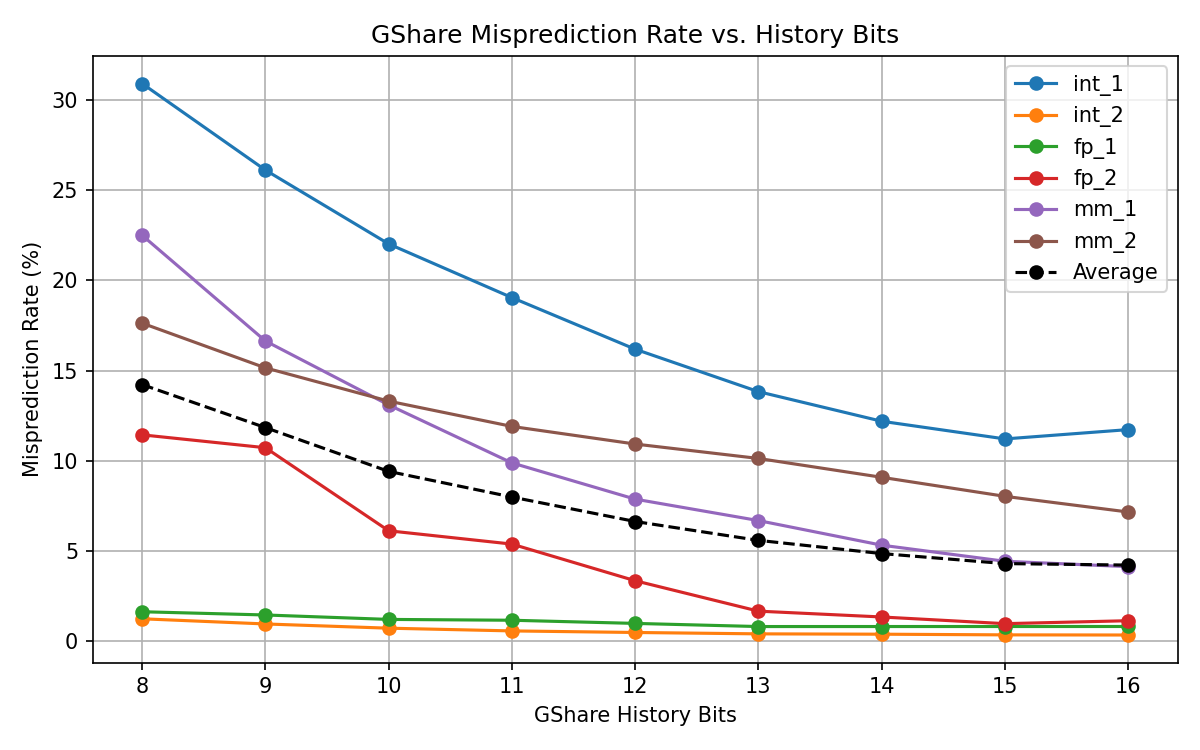
\includegraphics[width=\linewidth]{../gshare_sweep.png}
  \caption{G-Share Misprediction Rate vs. History Bits (8-16)}
  \label{fig:gshare_sweep}
  \Description{A line plot showing G-Share misprediction rate as a function of global history bits (from 8 to 16). Six lines represent the different traces, and one line shows the average. Misprediction generally decreases as history length increases.}
\end{figure}

\subsubsection{G-Share Parameter Sweep Analysis}
Figure \ref{fig:gshare_sweep} shows the effect of varying the GHR length from 8 to 16 bits. The "Average" line shows a clear trend: misprediction rates decrease as history length increases. This is expected, as longer history can distinguish more complex branch patterns. However, the gains diminish for very long histories, and for some traces like \texttt{int\_2}, performance is already so good that more history provides little benefit. For others like \texttt{int\_1}, longer history is crucial. This highlights the trade-off between performance and the exponentially increasing cost of the BHT.

\begin{figure*}[t]
  \centering
  \captionsetup{font=bf,size=small}
  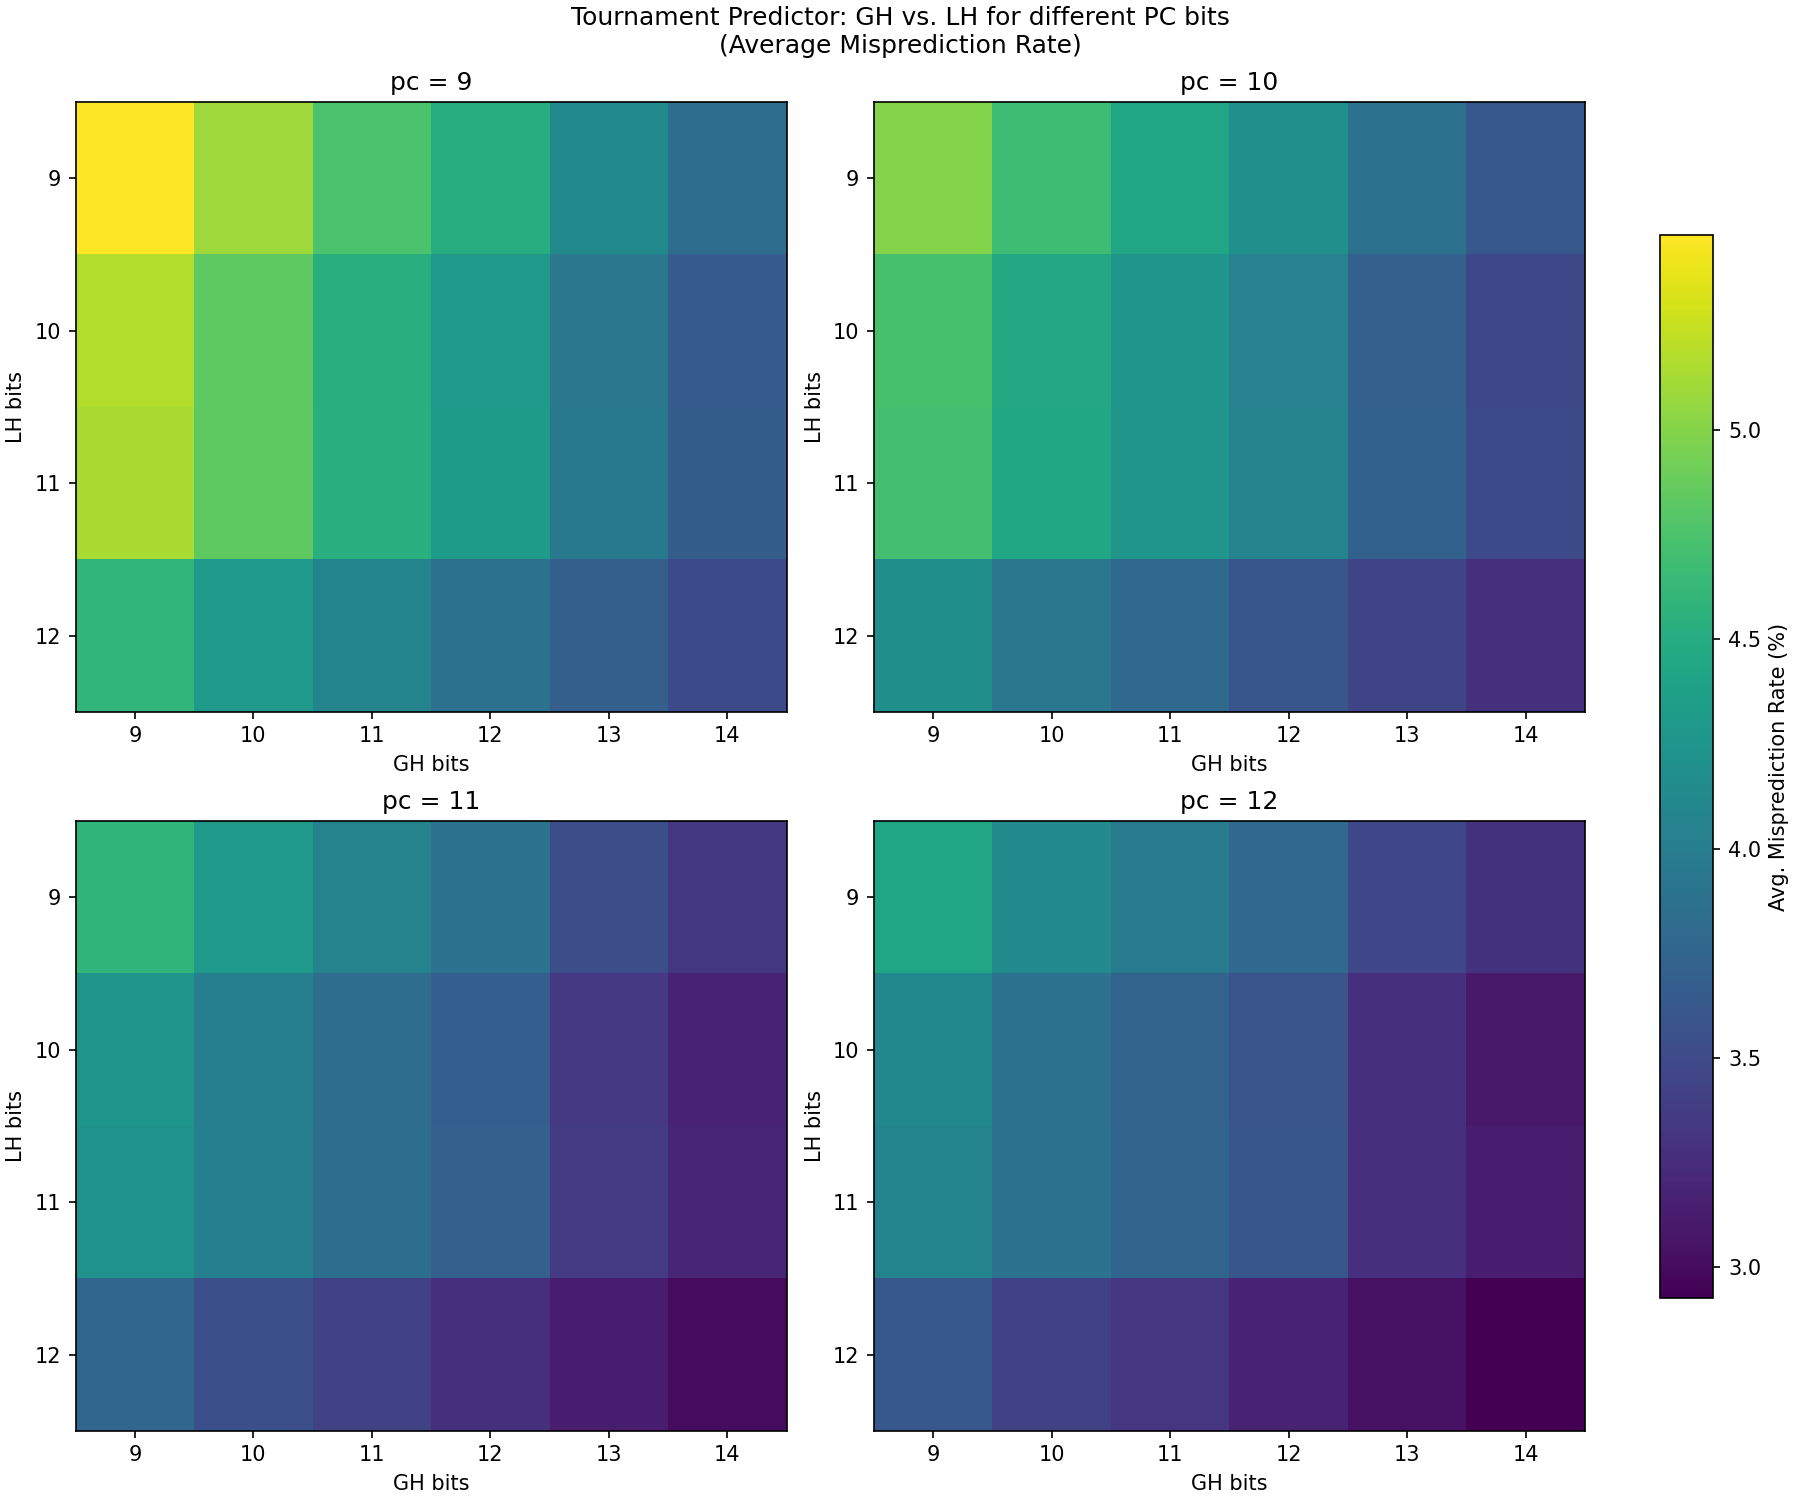
\includegraphics[width=0.8\textwidth]{../tournament_heatmap.png}
  \caption{Tournament Predictor: GH vs. LH for Different PC Bits (Average Misprediction Rate)}
  \label{fig:tourn_heatmap}
  \Description{Four heatmaps showing the average misprediction rate for the Tournament predictor. Each heatmap corresponds to a different number of PC index bits (9, 10, 11, 12). The x-axis is global history bits and the y-axis is local history bits. Darker purple/blue areas indicate lower misprediction rates.}
\end{figure*}

\subsubsection{Tournament Parameter Sweep Analysis}
Figure \ref{fig:tourn_heatmap} visualizes the three-dimensional design space of the Tournament predictor. Each subplot fixes the number of PC index bits and shows how the average misprediction rate varies with global history (GH) and local history (LH) bits.
\begin{itemize}
    \item \textbf{Impact of PC Index Bits:} Increasing the PC index bits (from pc=9 to pc=12) generally improves performance (the plots become darker overall). This is because a larger PC index for the local PHT reduces aliasing, allowing the local predictor to track more distinct branches accurately.
    \item \textbf{GH vs. LH Trade-off:} Within each plot, the optimal configurations (darkest regions) are not at the extremes. This indicates that a balance between local and global history is necessary. For example, in the pc=12 subplot, a configuration with high GH (13-14) and moderate LH (10-11) performs very well, suggesting that with aliasing reduced, global patterns become more valuable.
\end{itemize}
These heatmaps are powerful tools for a hardware designer to identify cost-effective configurations that yield high performance without over-allocating resources to any single component.

\section{Conclusion}

This project successfully implemented and evaluated three branch predictors of increasing complexity. Our findings provide a clear picture of the trade-offs between predictor design, hardware cost, and prediction accuracy.

\subsubsection{Summary of Findings}
\begin{itemize}
    \item The custom \textbf{TAGE predictor} demonstrated superior performance across all workloads, confirming that state-of-the-art academic predictors can deliver significant gains in practice. Its use of tagged, variable-length history is highly effective at capturing a wide range of branch behaviors while managing aliasing.
    \item The \textbf{Tournament predictor} serves as an excellent intermediate design, robustly handling diverse workloads by adapting between local and global strategies. It consistently outperforms G-Share, except in cases where workloads are heavily dominated by global correlations that benefit from a single, large global history table.
    \item \textbf{G-Share} remains a strong baseline, offering a substantial improvement over static prediction with minimal complexity. Its performance is highly sensitive to history length, but it provides a solid foundation for more advanced designs.
\end{itemize}

\subsubsection{Future Work}
This work could be extended in several promising directions:
\begin{itemize}
    \item \textbf{Perceptron Predictor:} Implement a perceptron-based predictor, which uses machine learning principles to weigh different features of branch history. This could offer a different approach to correlation and may excel on patterns TAGE finds difficult.
    \item \textbf{TAGE Enhancements:} Further tune the TAGE predictor by incorporating features from more recent designs, such as a loop predictor \cite{seznec2007tage} or a statistical corrector (SC) that leverages local history \cite{seznec2011}. A loop predictor would be particularly useful for highly regular, iterative branches, while a statistical corrector helps with branches that are statistically biased but not strongly correlated with global history.
    \item \textbf{Power and Latency Modeling:} The current study focuses on accuracy and memory size. A more complete analysis would involve modeling the latency and power consumption of each predictor to evaluate their overall efficiency in a realistic processor design.
\end{itemize}

%%
%% The acknowledgments section is defined using the "acks" environment
\begin{acks}
OpenAI's ChatGPT (model gpt-4o) was utilized to generate code from formulas and algorithms, assist in generating the visualization script to create plots from results, adding comments where needed, to help debug code and set up errors, and assist in \LaTeX formatting. The outputs from this AI model were modified with \textbf{major changes} to align with assignment requirements and ensure correctness. I actively reviewed, tested, and adjusted the generated code and explanations to reflect my own understanding.
\end{acks}

%%
%% The next two lines define the bibliography style to be used, and
%% the bibliography file.
\bibliographystyle{ACM-Reference-Format}
\bibliography{sample-base}


%%
%% If your work has an appendix, this is the place to put it.
\appendix
\section{Appendix: AI Tool Usage and Chat Logs}

\subsection{Overview}
In compliance with the project requirement to cite AI assistance and include prompts + outcomes, this appendix contains the key conversations with OpenAI’s ChatGPT (model gpt-4o). Below are excerpts showcasing how the tool was used to help debug code, generate example snippets, and provide explanatory text. All of these AI‐generated outputs were manually reviewed and substantially adapted.

\onecolumn
\subsection{Conversation 1: TAGE predictor counter debug}

\begin{Verbatim}[fontsize=\tiny, breaklines=true]
Me: I have a partially implemented TAGE predictor in C code, but I'm running into an issue where the saturating counter for the tagged entries sometimes goes out of range. Could you help me debug this?

GPT-4o: Absolutely, I'd be glad to help you debug your TAGE predictor implementation! The saturating counter going out of range is usually caused by incorrect updates (like incrementing beyond the max or decrementing below zero) or initialization issues.

To dig into it properly, could you share:

1. The relevant code snippet for your **TAGE table entry structure**, especially the saturating counter part.
2. The part of the code where you **update** the saturating counters.
3. The defined **limits** for your saturating counters (e.g., are they 2-bit? 3-bit?).

With that info, I can pinpoint exactly where the issue is. In the meantime, here are a few things you can check right away:

---

### Quick Checks for Debugging

1. **Counter Saturation Boundaries**:
   Make sure you're checking boundaries before updating:
   ```c
   if (entry.counter < MAX_COUNTER) {
       entry.counter++;
   }
   ```
   and
   ```c
   if (entry.counter > MIN_COUNTER) {
       entry.counter--;
   }
   ```

2. **Bit-width Constants**:
   If your counters are, say, 3-bit (i.e., range -4 to 3 for signed, or 0 to 7 for unsigned), verify that:
   - You’re using the correct type (signed vs. unsigned).
   - Your increments/decrements respect the upper/lower limits.

3. **Initialization**:
   Counters should be initialized to a neutral state, typically 0 or mid-range.

4. **Sign Confusion**:
   Are you using a signed saturating counter and treating it like an unsigned one (or vice versa)?

---

If you're not sure where the issue is, paste the key sections of your code here, and I’ll help you trace it step by step.

Me: Yeah here's the code:

```
static inline void tage_train(uint32_t pc, uint8_t outcome) {
    int needAllocate = 0;
    if (primaryBank < NUM_BANKS) {
        int8_t pCtr = tageBank[primaryBank].entry[ bankGlobalIndex[primaryBank] ].saturateCounter;
        // If mispredicted and the sign of pCtr is opposite the actual outcome => might allocate
        if ((lastPrediction != outcome) && ((pCtr >= 0) != outcome)) {
            needAllocate = 1;
        }
    } else {
        needAllocate = (lastPrediction != outcome);
    }

    if (needAllocate) {
        int8_t minUse = 127;
        for (int i = 0; i < primaryBank; i++) {
            int8_t u = tageBank[i].entry[ bankGlobalIndex[i] ].usefulness;
            if (u < minUse) {
                minUse = u;
            }
        }
        if (minUse > 0) {
            for (int i = primaryBank - 1; i >= 0; i--) {
                // This might decrement usefulness too aggressively without bound checks
                tageBank[i].entry[ bankGlobalIndex[i] ].usefulness--;
            }
        } else {
            int Y = rand() & ((1 << (primaryBank - 1)) - 1);
            int X = primaryBank - 1;
            while ((Y & 1) != 0) {
                X--;
                Y >>= 1;
                if (X < 0) break;
            }
            for (int i = X; i >= 0; i--) {
                if (tageBank[i].entry[ bankGlobalIndex[i] ].usefulness == minUse) {
                    // Re-init but never resets saturateCounter properly
                    tageBank[i].entry[ bankGlobalIndex[i] ].tag = generateGlobalEntryTag(pc, i);
                    tageBank[i].entry[ bankGlobalIndex[i] ].saturateCounter =
                        (outcome == TAKEN) ? 2 : -2; // Wrong initial range
                    tageBank[i].entry[ bankGlobalIndex[i] ].usefulness = 0;
                    break;
                }
            }
        }
    }

    // Directly increment/decrement saturateCounter with no range checks
    if (primaryBank < NUM_BANKS) {
        if (outcome == TAKEN) {
            tageBank[primaryBank].entry[ bankGlobalIndex[primaryBank] ].saturateCounter++;
        } else {
            tageBank[primaryBank].entry[ bankGlobalIndex[primaryBank] ].saturateCounter--;
        }
    } else {
        // update Bimodal (incorrectly – no bounding)
        int idx = pc % BIMODAL_SIZE;
        if (outcome == TAKEN) {
            t_bimodalPredictor[idx]++;
        } else {
            t_bimodalPredictor[idx]--;
        }
    }

    // If primary != alternate, we update the primary’s usefulness if we used it
    // (again without bounding, which can go out of range)
    if (lastPrediction != alternatePrediction) {
        if (primaryBank < NUM_BANKS) {
            if (lastPrediction == outcome) {
                tageBank[primaryBank].entry[ bankGlobalIndex[primaryBank] ].usefulness++;
            } else {
                tageBank[primaryBank].entry[ bankGlobalIndex[primaryBank] ].usefulness--;
            }
        }
    }

    // Shift in new outcome
    for (int i = MAX_HISTORY_LEN - 1; i > 0; i--) {
        t_globalHistory[i] = t_globalHistory[i - 1];
    }
    t_globalHistory[0] = outcome ? TAKEN : NOTTAKEN;

    // Update path history
    t_pathHistory <<= 1;
    t_pathHistory += (pc & 1);
    t_pathHistory &= ((1 << 16) - 1);

    // Update compressed histories (but missing some checks or re-initializations)
    for (int i = 0; i < NUM_BANKS; i++) {
        t_updateCompressed(&tageBank[i].indexCompressed, t_globalHistory);
        t_updateCompressed(&tageBank[i].tagCompressed[0], t_globalHistory);
        t_updateCompressed(&tageBank[i].tagCompressed[1], t_globalHistory);
    }
}
```

GPT-4o: Below is a rundown of what’s causing your **saturating counters** to go out of range in the snippet you posted and how to fix it. The main issues are:

1. **No Bound Checks** when incrementing or decrementing the saturating counters.  
2. **Re-initialization Values** (`+2` or `-2`) that may be inconsistent with the defined bit width of your counters.  
3. **Usefulness Counters** also updated without bounding, which can similarly wrap around.  

Let’s walk through the details.

---

## 1. Missing Bound Checks in Saturating Counter Updates

Right now, you do:
```c
if (outcome == TAKEN) {
    tageBank[primaryBank].entry[ bankGlobalIndex[primaryBank] ].saturateCounter++;
} else {
    tageBank[primaryBank].entry[ bankGlobalIndex[primaryBank] ].saturateCounter--;
}
```
with no checks. If you keep incrementing, you eventually push `saturateCounter` above the intended maximum; likewise, repeated decrementing can push it below the minimum. In an `int8_t`, once it passes `+127` or below `-128`, it wraps around, and your predictor logic breaks.

### **How to Fix**

1. **Decide the width** of your counters. Commonly in TAGE, each tagged entry uses a **3-bit** or **4-bit** signed saturating counter. For instance, if you use a **3-bit** scheme with sign-based prediction:
   - Negative values (-4 to -1) => “predict not taken”  
   - Zero or positive (0 to +3) => “predict taken”  
   - And you saturate at **-4** (min) or **+3** (max).  

2. **Clamp** on increment/decrement. For example, if using a 3-bit range of `-4..+3`:
   ```c
   #define MAX_CNT  3   // +3 is the maximum
   #define MIN_CNT -4   // -4 is the minimum

   int8_t *ctr = &tageBank[primaryBank].entry[ bankGlobalIndex[primaryBank] ].saturateCounter;
   if (outcome == TAKEN) {
       if (*ctr < MAX_CNT) {
           (*ctr)++;
       }
   } else {
       if (*ctr > MIN_CNT) {
           (*ctr)--;
       }
   }
   ```

That way, the counter does not exceed +3 or drop below -4, ensuring proper saturating behavior.

---

## 2. Re-Initializing the Counter to +2 or -2

Inside your “allocate” path, you do:
```c
tageBank[i].entry[ bankGlobalIndex[i] ].saturateCounter =
    (outcome == TAKEN) ? 2 : -2;  // Wrong initial range if 2-bit or mismatch
```
This can be **fine** if your saturating counter range is at least ±2. (In a 3-bit scheme from -4..+3, ±2 is valid and comfortably within the range.) However, if you intended to use only **2 bits** with sign-based logic, then the range is typically -2..+1 (four total states), and +2 would already be “out of range.”  

### **How to Fix**

- Confirm your desired saturating counter width and sign convention.  
- If it’s 3 bits (-4..+3), re-initializing to ±2 is perfectly valid. Just make sure your bounding constants match.  
- If it’s 2 bits (-2..+1), then you must clamp `+2` or `-2` to that narrower range.

---

## 3. No Bound Checks for Usefulness Counters

You also have a “usefulness” field:
```c
// This might decrement usefulness too aggressively without bound checks
tageBank[i].entry[ bankGlobalIndex[i] ].usefulness--;
```
and later:
```c
if (lastPrediction == outcome) {
    tageBank[primaryBank].entry[ bankGlobalIndex[primaryBank] ].usefulness++;
} else {
    tageBank[primaryBank].entry[ bankGlobalIndex[primaryBank] ].usefulness--;
}
```
If `usefulness` is supposed to be a small saturating counter (e.g., 2 bits or 3 bits), it can **wrap around** the same way as `saturateCounter`.

### **How to Fix**

- Decide the max/min for `usefulness` (e.g., 0..3).  
- Clamp it in exactly the same way:
  ```c
  #define U_MAX 3
  #define U_MIN 0

  if (tageBank[i].entry[ bankGlobalIndex[i] ].usefulness > U_MIN) {
      tageBank[i].entry[ bankGlobalIndex[i] ].usefulness--;
  }

  // Similarly for increment.
  ```

---

## 4. Bimodal Updates

In your bimodal branch:
```c
if (outcome == TAKEN) {
    t_bimodalPredictor[idx]++;
} else {
    t_bimodalPredictor[idx]--;
}
```
If `t_bimodalPredictor[idx]` is also a saturating counter (commonly 2 bits or 3 bits in a bimodal table), you must do the same saturating logic here:
```c
if (outcome == TAKEN) {
    if (t_bimodalPredictor[idx] < MAX_BIMODAL) {
        t_bimodalPredictor[idx]++;
    }
} else {
    if (t_bimodalPredictor[idx] > MIN_BIMODAL) {
        t_bimodalPredictor[idx]--;
    }
}
```

---

## Putting It All Together

**Key actions** to fix the out-of-range saturating counter bug:

1. **Define constants** for the saturating counter bounds.  
2. **Clamp** each increment/decrement to those bounds.  
3. Ensure your **initial values** (like +2 or -2) fall within the same bounds.  
4. Do the same for the **usefulness** counters and bimodal counters (if they’re also meant to be saturating).  

Once you add those fixes, you shouldn’t see the counters blowing past the valid range. Let me know if you have other questions on TAGE details, or if you need help deciding on the bit widths for your counters!
\end{Verbatim}

\subsection{Conversation 2: TAGE Predictor Overview}
\begin{Verbatim}[fontsize=\tiny, breaklines=true]
Me: Please provide a high-level explanation of how a TAGE predictor works, focusing on the multi-bank structure, the geometric history lengths, and how partial tags are generated.

GPT-4o: Sure! Here's a high-level explanation of how a **TAGE (TAgged GEometric history length) predictor** works, with a focus on its **multi-bank structure**, **geometric history lengths**, and **partial tag generation**:

---

### Overview of TAGE

TAGE is a **state-of-the-art branch predictor** used in modern CPUs to guess the direction of branches (taken or not taken) before they're resolved, improving instruction-level parallelism. It builds on the idea that **longer branch histories** can improve prediction accuracy, but in a smart and scalable way.

---

### Multi-bank Structure

- TAGE uses **multiple predictor components**, often called **banks or tables**.
- Each table (except for the base one) is associated with a **different history length**, forming a hierarchy.
- The predictor uses **one base predictor** (often a simple bimodal predictor) and several **tagged predictor tables**.
- Each tagged table is indexed using a **compressed version** of the global branch history, allowing it to capture correlations over different history lengths.

**Key idea**: If a long history length yields a confident prediction, use it. Otherwise, fall back to shorter histories or the base predictor.

---

### Geometric History Lengths

- Each tagged table uses a **different history length**, forming a **geometric progression**:
  ```
  L(i) = floor(\alpha^i), for i = 0 to N-1
  ```
  where:
  - `L(i)` is the history length for table `i`
  - `\alpha` is a geometric growth factor (e.g., 1.5 to 2)
  - `N` is the number of tagged tables
- This setup allows TAGE to cover a wide range of history lengths with **fewer tables**, efficiently balancing coverage and resource usage.

---

### Partial Tag Generation

- Each entry in a tagged table stores a **partial tag** to match against the branch’s history-derived signature.
- A **partial tag** is generated by:
  - **Hashing or folding** the program counter (PC) and the global history into a small number of bits.
  - This allows a small tag to identify whether a prediction entry corresponds to the current branch and history pattern.
- Partial tags help **differentiate between branches** that may map to the same table entry (avoiding aliasing errors).

---

### Prediction Process

1. For a given branch:
   - The PC and global history are used to index all tables.
   - The predictor searches for the **longest history match** among the tables.
2. If a match is found (tag matches), the prediction from that table is used.
3. If no match, the base predictor is used.
4. If two or more matches exist, the **longest matching history** wins.

---

### Summary

- **Multi-bank structure**: Multiple tables store predictions with varying history lengths.
- **Geometric history lengths**: History lengths grow exponentially to capture both short-term and long-term correlations.
- **Partial tags**: Small hash-like signatures identify valid entries for a given PC/history pair.

Let me know if you want a diagram or a more detailed example to go with this!
\end{Verbatim}

\subsection{Conversation 3: TAGE predictor bit calculation}
\begin{Verbatim}[fontsize=\tiny, breaklines=true]
Me: I'm trying to keep my TAGE predictor under 64K + 256 bits. How do I calculate the bit usage for each bank if I have 3 bits for the saturating counter, 10 bits for the tag, and 2 or 3 bits for usefulness? Also, how do I account for compressed histories?

GPT-4o: Great question! Let's break this down and calculate the storage used per entry in each TAGE bank, and then look at how to stay within your budget of **64K + 256 bits** (which is **65,280 bits** total).

---

### **Per-Entry Bit Usage (per bank)**

For **each TAGE predictor bank entry**, you typically store:

1. **Tag** = 10 bits  
2. **Saturating Counter** = 3 bits  
3. **Usefulness Counter** = 2 or 3 bits (depends on your design)  

So per entry:
- If 2-bit usefulness: `10 + 3 + 2 = 15 bits`
- If 3-bit usefulness: `10 + 3 + 3 = 16 bits`

---

### **Compressed Histories**

**Compressed histories** are used to save storage on the history-based indexing and tagging functions. These aren't per-entry — they’re global/shared across banks.

- You typically store a **compressed history** for each bank, used in indexing and tagging. The size of each compressed history depends on:
  - The global history length used
  - Number of banks
  - The folding strategy

In many designs, each compressed history is ~10–16 bits per component (depending on folding), and you may have:
- One for index generation (per bank)
- One for tag generation (per bank)

So rough estimate:  
`~2 compressed histories × N banks × ~16 bits = small amount`  
Say for 8 banks: `2 × 8 × 16 = 256 bits` — which actually matches the **+256** in your `64K + 256` constraint.

**Conclusion:** You’re allowed to spend **64K bits (65,024 bits)** on your *tables*, and the extra 256 bits are for compressed histories.

---

### **Storage Budget Summary**

You have:
- **64K bits = 65,024 bits for TAGE entries**
- **+256 bits for compressed histories**

Let’s calculate how many entries you can have per bank.

---

### **Example: How Many Entries per Bank?**

Let’s say:
- 4 banks
- Usefulness counter = 2 bits
- So each entry = 15 bits

Assuming equal size per bank:
```
Total bits per bank = 65,024 / 4 = 16,256 bits
Entries per bank = 16,256 / 15 \approx 1,083 entries
```

If usefulness = 3 bits (16 bits per entry):
```
Entries per bank = 16,256 / 16 = 1,016 entries
```

You can also vary the number of entries per bank (fewer entries for longer-history banks).

---

### Other Considerations:

- **Base Predictor**: Don’t forget that TAGE usually includes a base predictor (like a bimodal table), which may need separate bits.
- **Banked vs Fully Associative**: If you implement associativity or partial associativity, it affects indexing and possibly tag size.
- **Replacement Information**: If you store any replacement priority bits, you’ll need to include those too.

---

### TL;DR:

- **Per-entry size = tag (10) + ctr (3) + useful (2–3) = 15–16 bits**
- **Compressed histories \approx 256 bits total — fits within the “+256 bits” budget**
- Use your total bit budget (65,024) to divide across banks and determine entry count

Let me know how many banks you’re using or if you want help optimizing your layout!
\end{Verbatim}

\subsection{Conversation 4: TAGE Training Function Annotation}
\begin{Verbatim}[fontsize=\tiny, breaklines=true]
Me: 

Could you annotate the tage_train() function?

static inline void tage_train(uint32_t pc, uint8_t outcome) {
    int needAllocate = 0;
    if (primaryBank < NUM_BANKS) {
        int8_t pCtr = tageBank[primaryBank].entry[ bankGlobalIndex[primaryBank] ].saturateCounter;
        // If mispredicted and the sign of pCtr is opposite the actual outcome => might allocate
        if ((lastPrediction != outcome) && ((pCtr >= 0) != outcome)) {
            needAllocate = 1;
        }
    } else {
        needAllocate = (lastPrediction != outcome);
    }

    if (needAllocate) {
        int8_t minUse = 127;
        for (int i = 0; i < primaryBank; i++) {
            int8_t u = tageBank[i].entry[ bankGlobalIndex[i] ].usefulness;
            if (u < minUse) {
                minUse = u;
            }
        }
        if (minUse > 0) {
            for (int i = primaryBank - 1; i >= 0; i--) {
                tageBank[i].entry[ bankGlobalIndex[i] ].usefulness--;
            }
        } else {
            int Y = rand() & ((1 << (primaryBank - 1)) - 1);
            int X = primaryBank - 1;
            while ((Y & 1) != 0) {
                X--;
                Y >>= 1;
                if (X < 0) break;
            }
            for (int i = X; i >= 0; i--) {
                if (tageBank[i].entry[ bankGlobalIndex[i] ].usefulness == minUse) {
                    // Re-init
                    tageBank[i].entry[ bankGlobalIndex[i] ].tag = generateGlobalEntryTag(pc, i);
                    tageBank[i].entry[ bankGlobalIndex[i] ].saturateCounter =
                        (outcome == TAKEN) ? 0 : -1;
                    tageBank[i].entry[ bankGlobalIndex[i] ].usefulness = 0;
                    break;
                }
            }
        }
    }

    // Update the saturating counter
    if (primaryBank < NUM_BANKS) {
        updateSaturate(
            &tageBank[primaryBank].entry[ bankGlobalIndex[primaryBank] ].saturateCounter,
            outcome,
            LEN_COUNTS
        );
    } else {
        // update Bimodal
        int idx = pc % BIMODAL_SIZE;
        updateSaturateMinMax(&t_bimodalPredictor[idx], outcome, 0, (1 << LEN_BIMODAL) - 1);
    }

    // If primary != alternate, we update the primary’s usefulness if we used it
    if (lastPrediction != alternatePrediction) {
        if (primaryBank < NUM_BANKS) {
            updateSaturateMinMax(
                &tageBank[primaryBank].entry[ bankGlobalIndex[primaryBank] ].usefulness,
                (lastPrediction == outcome),
                0, 3
            );
        }
    }

    // Shift in new outcome
    for (int i = MAX_HISTORY_LEN - 1; i > 0; i--) {
        t_globalHistory[i] = t_globalHistory[i - 1];
    }
    t_globalHistory[0] = outcome ? TAKEN : NOTTAKEN;

    // Update path history
    t_pathHistory <<= 1;
    t_pathHistory += (pc & 1);
    t_pathHistory &= ((1 << 16) - 1);

    // Update compressed histories
    for (int i = 0; i < NUM_BANKS; i++) {
        t_updateCompressed(&tageBank[i].indexCompressed, t_globalHistory);
        t_updateCompressed(&tageBank[i].tagCompressed[0], t_globalHistory);
        t_updateCompressed(&tageBank[i].tagCompressed[1], t_globalHistory);
    }
}

GPT-4o: Below is an annotated version of the `tage_train()` function. The annotations are placed as comments before or alongside relevant sections of the code to explain the purpose and logic behind each step.

---

```cpp
static inline void tage_train(uint32_t pc, uint8_t outcome) {
    // 1. Determine whether we need to allocate a new entry in the TAGE tables (i.e., whether
    //    the prediction was mispredicted and we have reason to believe a new entry could
    //    improve future prediction accuracy).

    int needAllocate = 0;

    // primaryBank is the TAGE bank (or set of banks) that provided the final prediction.
    // If primaryBank is valid (less than NUM_BANKS), we have a prediction from TAGE.
    // Otherwise, the prediction came from the bimodal predictor.
    if (primaryBank < NUM_BANKS) {
        // pCtr is the saturating counter from the TAGE table entry in the primary bank.
        int8_t pCtr = tageBank[primaryBank].entry[ bankGlobalIndex[primaryBank] ].saturateCounter;

        // If the final prediction was wrong AND the sign of pCtr is opposite from the actual outcome,
        // we may want to allocate a new entry from the other TAGE banks (which didn't match).
        // This is a typical "allocate on misprediction" strategy for TAGE.
        if ((lastPrediction != outcome) && ((pCtr >= 0) != outcome)) {
            needAllocate = 1;
        }
    } else {
        // If the prediction was from the bimodal predictor, we consider allocating
        // if the prediction was simply incorrect.
        needAllocate = (lastPrediction != outcome);
    }

    // 2. If we need to allocate, determine whether it is possible or desirable to do so.
    //    TAGE banks use a "usefulness" counter to decide if an entry is worth replacing.

    if (needAllocate) {
        int8_t minUse = 127;

        // Search for the minimum "usefulness" across all banks that are more selective (i.e. < primaryBank).
        // The lower this value, the more likely it is that an entry can be replaced.
        for (int i = 0; i < primaryBank; i++) {
            int8_t u = tageBank[i].entry[ bankGlobalIndex[i] ].usefulness;
            if (u < minUse) {
                minUse = u;
            }
        }

        // If all banks have high usefulness, we decrement the usefulness counters (to give a chance
        // for entries to become less useful and thus replaceable in the future).
        if (minUse > 0) {
            for (int i = primaryBank - 1; i >= 0; i--) {
                tageBank[i].entry[ bankGlobalIndex[i] ].usefulness--;
            }
        } else {
            // Otherwise, at least one bank has minimal usefulness, and we can replace an entry in one of
            // those banks with a new tag/saturating counter.

            // Y is used here to randomly select which bank (among the possible ones) gets the new entry.
            // The expression "(1 << (primaryBank - 1)) - 1" essentially creates a bitmask. 
            // For example, if primaryBank = 3, we get (1 << 2) - 1 = 3 (binary 11).
            int Y = rand() & ((1 << (primaryBank - 1)) - 1);
            int X = primaryBank - 1;

            // This loop steps backward through the banks (less selective to more selective) until it
            // finds one that is randomly selected to allocate.
            while ((Y & 1) != 0) {
                X--;
                Y >>= 1;
                if (X < 0) break;
            }

            // Once we choose bank X, look for an entry in that bank with usefulness == minUse.
            // We then re-initialize it with the new tag, a saturating counter biased by the outcome,
            // and reset usefulness.
            for (int i = X; i >= 0; i--) {
                if (tageBank[i].entry[ bankGlobalIndex[i] ].usefulness == minUse) {
                    // Re-initialize the entry with the new tag and starting counter value.
                    tageBank[i].entry[ bankGlobalIndex[i] ].tag = generateGlobalEntryTag(pc, i);
                    tageBank[i].entry[ bankGlobalIndex[i] ].saturateCounter =
                        (outcome == TAKEN) ? 0 : -1;
                    tageBank[i].entry[ bankGlobalIndex[i] ].usefulness = 0;
                    break;
                }
            }
        }
    }

    // 3. Update the saturating counter in the primary bank (if used), or the bimodal predictor (otherwise).
    //    Saturating counters move up/down based on whether the outcome was TAKEN or NOTTAKEN.
    if (primaryBank < NUM_BANKS) {
        updateSaturate(
            &tageBank[primaryBank].entry[ bankGlobalIndex[primaryBank] ].saturateCounter,
            outcome,
            LEN_COUNTS
        );
    } else {
        // If the prediction came from the bimodal predictor, update it instead.
        int idx = pc % BIMODAL_SIZE;
        updateSaturateMinMax(&t_bimodalPredictor[idx], outcome, 0, (1 << LEN_BIMODAL) - 1);
    }

    // 4. If the primary prediction was different from the alternate prediction,
    //    update the usefulness counter for the primary table’s entry. We reward or penalize
    //    the primary TAGE entry if it got the actual outcome right or wrong, respectively.
    if (lastPrediction != alternatePrediction) {
        if (primaryBank < NUM_BANKS) {
            updateSaturateMinMax(
                &tageBank[primaryBank].entry[ bankGlobalIndex[primaryBank] ].usefulness,
                (lastPrediction == outcome),
                0, 3
            );
        }
    }

    // 5. Update the global history with the new outcome. This shifts the array t_globalHistory
    //    and inserts the latest taken/not-taken result at the front (index 0).
    for (int i = MAX_HISTORY_LEN - 1; i > 0; i--) {
        t_globalHistory[i] = t_globalHistory[i - 1];
    }
    t_globalHistory[0] = outcome ? TAKEN : NOTTAKEN;

    // Update the path history (which often tracks the program-counter's least significant bits).
    t_pathHistory <<= 1;
    t_pathHistory += (pc & 1);
    t_pathHistory &= ((1 << 16) - 1); // keep only the lower 16 bits

    // 6. Update the compressed histories for each TAGE bank. Compressed history is used to index
    //    and tag TAGE tables with partial, hashed versions of the global history.
    for (int i = 0; i < NUM_BANKS; i++) {
        t_updateCompressed(&tageBank[i].indexCompressed, t_globalHistory);
        t_updateCompressed(&tageBank[i].tagCompressed[0], t_globalHistory);
        t_updateCompressed(&tageBank[i].tagCompressed[1], t_globalHistory);
    }
}
```

### Summary of Key Points

1. **`needAllocate`:** Determines if the predictor will attempt to allocate a new entry in TAGE for better prediction in the future. This is triggered by a misprediction and a sign mismatch between the saturating counter and the actual outcome.

2. **Usefulness Counters:** TAGE uses “usefulness” to determine if an entry is likely still relevant. If no entries can be replaced (i.e., all have high usefulness), the predictor decrements usefulness counters to eventually free them for re-allocation.

3. **Random Replacement Among Candidates:** If multiple entries are at minimum usefulness, TAGE randomly chooses which one to replace. This helps spread out the chance of finding a beneficial new entry.

4. **Updating Saturating Counters:** After each prediction, the saturating counter is updated to reflect the actual outcome, so the same pattern in the future can be predicted more accurately.

5. **Usefulness Update:** If the primary TAGE bank disagreed with the alternate but was correct, we increase its usefulness (and vice versa).

6. **Updating History:** Global history (`t_globalHistory`), path history (`t_pathHistory`), and compressed history are all updated with the latest outcome to keep the TAGE tables properly indexed and tagged for future predictions.
\end{Verbatim}

\subsection{Conversation 5: Docker setup for predictor}
\begin{Verbatim}[fontsize=\tiny, breaklines=true]
Me: Show me how to set up a Docker container to compile and run `predictor.c` with `make`. I'm on Windows, so I might need the correct volume mounts. Also show me the exact commands I'd run to test the .bz2 trace files in my trace/ dir.

GPT-4o: Sure! Let's walk through setting up a Docker container that compiles and runs `predictor.c` using `make`, and also lets you test `.bz2` trace files from a `trace/` directory on your Windows machine.

---

## Step 1: Project Layout (Assumed)

Suppose your project folder looks like this on your **Windows host**:

```
C:\Users\YourName\branch_predictor\
│
├── predictor.c
├── Makefile
├── sim
├── trace\
│   ├── trace1.bz2
│   └── trace2.bz2
```

We'll mount this directory into Docker.

---

## Step 2: Create a Dockerfile (optional)

If you want a custom environment, create a `Dockerfile` like this:

```Dockerfile
FROM ubuntu:22.04

# Install build tools and bunzip2
RUN apt update && apt install -y build-essential bzip2

WORKDIR /app
```

Build it with:

```bash
docker build -t predictor-env .
```

Alternatively, you can skip this and use a base image like `gcc` with bzip2.

---

## Step 3: Run Docker with Proper Mounts

On **Windows**, your path `/mnt/c/Users/YourName/branch_predictor` corresponds to `C:\Users\YourName\branch_predictor`.

Here’s the Docker run command:

```bash
docker run --rm -it -v /mnt/c/Users/YourName/branch_predictor:/app -w /app predictor-env bash
```

Or, if you didn’t build a custom image:

```bash
docker run --rm -it -v /mnt/c/Users/YourName/branch_predictor:/app -w /app ubuntu:22.04 bash
```

Then install the tools inside the container:

```bash
apt update
apt install -y build-essential bzip2
```

---

## Step 4: Compile with Make

Inside the container (you're now at `/app`, which is your Windows project dir):

```bash
make
```

This should compile `predictor.c` into the binary `sim`.

---

## Step 5: Run Sim with `.bz2` Trace Files

Assuming `sim` takes a trace file as argument like this:

```bash
./sim -t trace/trace1.bz2
```

You can run any of the traces like:

```bash
./sim -t trace/trace1.bz2
./sim -t trace/trace2.bz2
```

If you want to loop over them:

```bash
for f in trace/*.bz2; do
  ./sim -t "$f"
done
```

---

## Full Session Recap (All Together)

```bash
docker run --rm -it -v /mnt/c/Users/YourName/branch_predictor:/app -w /app ubuntu:22.04 bash

# In Docker:
apt update
apt install -y build-essential bzip2
make
./sim -t trace/trace1.bz2
```

---

Would you like help writing a `Makefile`, if you don't already have one? Or a script to automate all trace testing?
\end{Verbatim}

\subsection{Conversation 6: Gshare Misprediction Rate Difference}
\begin{Verbatim}[fontsize=\tiny, breaklines=true]
Me: Can you explain why the runall.sh script outputs "Misprediction Rate: 0.826" for gshare:14 on fp_1 but "Misprediction Rate: 0.827" for gshare:15? Are those differences from random seeds or actual structural differences in the table indexing?

GPT-4o: The slight difference in **Misprediction Rate** between `gshare:14` (0.826) and `gshare:15` (0.827) is most likely due to **actual structural differences in the indexing mechanism** of the **gshare** predictor, rather than random seeds — assuming the simulator is deterministic (most academic simulators are).

Let me break it down for you:

---

### What is gshare?

**gshare** is a dynamic branch predictor that uses:

- **Global History Register (GHR)**: tracks outcomes of recent branches.
- **Program Counter (PC)**: identifies the current branch.
- These two are XOR’ed together to generate an **index** into a **prediction table** (Pattern History Table or PHT).

---

### What does `gshare:14` or `gshare:15` mean?

These likely refer to the number of **index bits** used to access the prediction table:
- `gshare:14` → 14 bits are used to index the table.
- `gshare:15` → 15 bits are used.

This affects:
- **Table size** (2¹⁴ vs. 2¹⁵ entries).
- **Indexing behavior**, because more bits from the PC and GHR are used in the XOR.

---

### Why the slight difference?

1. **Structural behavior:**
   - A larger table (`gshare:15`) generally helps — more entries, less aliasing.
   - But it can also cause **different aliasing patterns**: more bits from the GHR and PC are involved, and the way they XOR may group branches differently.
   - This can cause **some branches to benefit** and others to suffer, especially on specific traces like `fp_1`.

2. **Trace sensitivity:**
   - The `fp_1` trace might have branch patterns that align better with 14 bits than 15 due to its structure or frequency of certain PCs.

3. **Rounding error?**
   - If the misprediction rate is output as a **rounded float**, e.g. 0.826 vs. 0.827, the actual raw numbers might be very close, like:
     - `0.8264` (rounded to 0.826)
     - `0.8265` (rounded to 0.827)

---

### Is randomness involved?

Unlikely unless:
- The simulator is non-deterministic (e.g., uses random initial table values or thread interleaving).
- You’re using randomized inputs or seeds (e.g., in a neural predictor or ML-based branch predictor — not typical for gshare).

If you're using a standard gshare implementation and always run the same trace (`fp_1`), the results should be deterministic.

---

### Summary:

The difference in misprediction rate between `gshare:14` and `gshare:15` is due to **structural indexing differences** (how GHR and PC bits XOR to select table entries), not randomness. The slightly worse rate for `gshare:15` on `fp_1` is probably a quirk of **aliasing patterns** or rounding precision — not an anomaly.

If you want, I can show you how to visualize the indexing to see exactly which bits are used at each size.
\end{Verbatim}

\thispagestyle{ack_footer}


\end{document}
\endinput
%%
%% End of file